%!TEX root = ..\main.tex
\section{Langevin Dynamics}
\label{sec:langevin_dynamics}

\subsection{Langevin equations}
\label{subsec:langevin_equations}
To study dynamics of system described in section \ref{sec:model}, we apply the Langevin dynamics approach, which follows the Langevin equation of (translational) motion
\begin{equation}
\label{eq:langevin_theory_1}
	\dot{r} = v
\end{equation}
\begin{equation}
\label{eq:langevin_theory_2}
	m \dot{v} = f(r, t) - \alpha v + \beta(t)
\end{equation}
where $\alpha$ is damping coefficient related with a drag force induced by a medium, and $f(r, t)$ is a force acting on a particle. $\beta$ is a stochastic force, and in order to satisfy dissipation-fluctuation theorem, it is assumed to be Gaussian-distributed, with
\begin{equation}
\langle\beta(t)\rangle = 0,
\end{equation}
\begin{equation}
\label{eq:stochastic_term_dispersion}
\langle\beta(t)\beta(t')\rangle = 2 \alpha k_B T\delta(t - t')
\end{equation}
where $k_B$ is the Boltzmann constant, $T$ is thermostat temperature, $\delta$ is the Dirac delta function and the average is done over ensemble of particles.

For the rotational motion the form of equations remains unchanged, but one have to do a direct substitution of 
\begin{equation}
\label{eq:rotation_translation_substitution}
	\begin{aligned}[c]
		\phi &\rightarrow r        \\
		\omega &\rightarrow v 
	\end{aligned}
	\qquad
	\qquad
	\begin{aligned}[c]
		I &\rightarrow m        \\
		\tau(r, t) &\rightarrow f(r, t)
	\end{aligned}
\end{equation}
where $\phi$ is particle orientation angles, $\omega$ is angular velocity, $I$ is inertia and $\tau$ is torque exerted on a particle.

The damping coefficients $\alpha$ for translation ($\alpha_t$) and rotation ($\alpha_r$) are different, and can be obtained in following way.

First to simplify the particle-solution interaction description we need to define damping time $\tau$, which determines how rapidly decays thermal fluctuations in particles positions and orientations \textcolor{red}{Or what is the proper way of saying that it shows how dense is surrounding media?}, and for translational motion it is given by
\begin{equation}
\label{eq:Translation_damping_time}
	\tau_{t} = \frac{m}{6 \pi \eta R}
\end{equation}
where $m$ is particle mass, $\eta$ is viscosity and $R$ is particle radius. For rotation $\tau_{t} / \tau_{r} = 10/3$, which can be obtained from Stokes-Einstein-Debye relations Eqs.~\eqref{eq:translational_diffusion_coefficient}~and~\eqref{eq:rotational_diffusion_coefficient}. and relation between particle mass and inertia.

And then the $\alpha_t$ and $\alpha_r$ are defined
\begin{equation}
	\begin{aligned}
		\alpha_t = \frac{m}{\tau_t}
	\end{aligned}
	\qquad
	\qquad
	\begin{aligned}
		\alpha_r = \frac{I}{\tau_r}
	\end{aligned}
\end{equation}
where $m$ is particle mass, $I$ is inertia, $\tau_{t,r}$ are damping times.

\subsection{Integration method}
\label{subsec:integration_method}

The integration scheme for translational equations of motion proposed in~\cite{Taylor2013} is as follows
\begin{equation}
\label{eq:tr_coordinate_change}
	r^{n+1} = r^n + dt \left(
	 b_{t} v^n
	 + \frac{b_{t} dt}{2m}f^n
	 + \frac{b_{t}}{2m}\beta_{t}^{n+1}
	\right)
\end{equation}
\begin{equation}
\label{eq:tr_velocity_change}
	v^{n+1} = v^n 
	 + \frac{dt}{2m}\left(f^n + f^{n+1}\right)
	 - \frac{\alpha_{t}}{m}\left(r^{n+1} - r^n\right)
	 + \frac{1}{m}\beta_{t}^{n+1}
\end{equation}

The same integration scheme can be used for rotation, with proper change of variables (see Eq.~(\ref{eq:rotation_translation_substitution}))
\begin{equation}
\label{eq:rot_angle_change}
	\phi^{n+1} = \phi^n + dt \left(
	  b_{r} \omega^n
	  + \frac{b_{r} dt}{2I}\tau^n
	  + \frac{b_{r} }{2I}\beta_{r}^{n+1}
	 \right)
\end{equation}
\begin{equation}
\label{eq:rot_ang_velocity_change}
	\omega^{n+1} = \omega^n
	+ \frac{dt}{2m}\left(\tau^n + \tau^{n+1}\right)
	- \frac{\alpha_{r}}{I}\Delta u
	+ \frac{1}{I}\beta_{r}^{n+1}
\end{equation}
here $\Delta u \equiv \left(\phi^{n+1} - \phi^n\right)$ is rotation of the particle within one integration step. Vector $\Delta u$ is parallel to the axis around which particle has rotated on the angle $|\Delta u|$ radians. The coefficients $b_t$ and $b_r$ accounts for the drag exerted on a particle by surrounding medium,
\begin{equation}
\label{eq:drag_coefficient}
	\begin{aligned}
		b_t = \frac{1}{1 + \frac{\alpha_t dt}{2 m}}
	\end{aligned}
	\qquad
	\qquad
	\begin{aligned}
		b_r = \frac{1}{1 + \frac{\alpha_r dt}{2 I}}
	\end{aligned}
\end{equation}

When $\alpha_{tr} = 0$, from Eq.~\eqref{eq:drag_coefficient} we obtain $b_{tr} = 1$ and from Eq.~\eqref{eq:stochastic_term_dispersion} we obtain $\langle\beta_{tr}(t)\beta_{tr}(t')\rangle = 0$. Then the above equations reduces to the standard velocity-Verlet scheme \textcolor{red}{I understand that $\alpha = 0$ is frictionless regime? I should say it directly?}\textcolor{yellow}{i am not sure how physical it is... as without drag you should also not have a stochastic term...}\textcolor{red}{Yes, you are totally right. With $\alpha = 0$ the stochastic term has zero dispersion because $\alpha$ is also in Eq. \ref{eq:stochastic_term_dispersion}} The damping is calculated as integral  over real path travelled by particle within time step (under assumption that damping time does not change within $dt$ and $\Delta r$).

If using integration scheme defined in eq. (\ref{eq:rot_angle_change}), effective angular velocity of a particle within every time step is
\begin{equation}
\label{eq:effective_angular_velocity}
	\tilde{\omega}^n = b_{r} \omega^n
	+ \frac{b_{r} dt}{2I}\tau^n
	+ \frac{b_{r} }{2I}\beta_{r}^{n+1}
\end{equation}

By the definition, angular velocity $\tilde{\omega}^n$ is directed parallel to the axis around which particle is rotated on the angle $|\tilde{\omega}^n|dt$ per time step $dt$. Therefore, if particle orientation is defined by quaternion $q$, then the Eq.~\eqref{eq:rot_angle_change} can be written like
\begin{equation}
q^{n+1} = \tilde{q}\,^n q^{n}
\end{equation}
where $q^n$ and $q^{n+1}$ is the quaternion representation of orientation on time steps $n$ and $n+1$ respectively, and $\tilde{q}\,^n q^{n}$ is quaternion multiplication. \textcolor{red}{quaternions defined in appendix}. $\tilde{q}\,^n$ is the quaternion representation of rotation around $\tilde{\omega}^n$ on the angle $|\tilde{\omega}^n|$.

\subsection{Interactions}

To perform simulations we need to define forces acting on the particles.

First of all, as in the Monte-Carlo simulations we restrict interactions to the immediate neighbors (particle $i$ interacts only with particles $i+1$ and $i-1$).

The force acting on a particle is defined by gradient of potential energy.
\begin{equation}
\label{eq:full_force}
	\vec{F}_{ij}
		= -\frac{\delta E_{ij}}{\delta \vec{r}}
		=  \frac{\hat{r}}{r^4} \left[3 D - A\, r^2 (k r +1) \, \exp(-k r) \right]
\end{equation}
where $D = 3 \cos \theta_1 \cos \theta_2 - (\hat{m}_1 \cdot \hat{m}_2)$ stands for orientational part of dipole-dipole potential, $\vec{r}$ is distance between particle centers. The other parameters are the same as in Eqs.~\eqref{eq:dipole_dipole_1D}~and~eq.~\eqref{eq:yukawa_interaction}

The torque on a particle arises only due to dipole-dipole interaction. Therefore it is calculated as
\begin{equation}
\label{eq:dipole_torque}
	\vec{\tau}  = \mu[\hat{\mu} \times \vec{E}_d ]
\end{equation}
where $\vec{\mu}$ is dipole moment of particle on which torque acts, and $\vec{E}_d$ is dipole field produced by acting particle.

\begin{equation}
\label{eq:dipole_field}
	\vec{E}_d = \frac{\mu}{r^3}
		\left(3 (\hat{\mu} \cdot \hat{r}) \hat{r} - \hat{\mu} \right)
\end{equation}
where $\mu$ is dipole moment of the particle inducing the field.

\subsection{Statistical properties}
For non-interacting spheres the relation between rotational and translational diffusion coefficient can be obtained \cite{C5SM02754C}. The former is given by the Stokes-Einstein relation
\begin{equation}
\label{eq:translational_diffusion_coefficient}
	D_t = \frac{k_B T}{6 \pi \eta R}
\end{equation}
and the latter is given by Stokes-Einstein-Debye relation
\begin{equation}
\label{eq:rotational_diffusion_coefficient}
	D_r = \frac{k_B T}{8 \pi \eta R^3}
\end{equation}
where $T$ is temperature, $\eta$ the viscosity of the fluid medium and $k_B$ the Boltzmann constant. The relation between $D_t$ and $D_r$ is given by
\begin{equation}
	\frac{D_r}{D_t} = \frac{3}{4 R^2}
\end{equation}

For sufficiently long times, we can estimate the diffusion coefficient as
\begin{equation}
\label{eq:translation_diffusion_vs_displacement}
	D_t = \lim_{\Delta t \to \infty} \frac{1}{6 \Delta t} \langle r^2(\Delta t)\rangle
\end{equation}
where $\langle r^2(\Delta t)\rangle$ is translational mean square displacement (MSD) of particle relatively to its initial position,
\begin{equation}
	\langle r^2(\Delta t)\rangle
	 = \frac{1}{N} \sum_{i=1}^{N} |\vec{r}_i(t + \Delta t) - \vec{r}_i(t)|^2
\end{equation}

Analogously can be defined relation between rotational diffusion coefficient $D_r$ and rotational mean square displacement (RMSD) $\langle \phi^2(\Delta t) \rangle$
\begin{equation}
\label{eq:rotational_diffusion_vs_displacement}
	D_r = \lim_{\Delta t \to \infty} \frac{1}{6 \Delta t} \langle \phi^2(\Delta t)\rangle
\end{equation}
\textcolor{red}{I've decided that that previous way of calculating displacement was overly complicated, so I've replaced it with quaternions. Works 3 times faster and gives same results}
The vector $\Delta u$ of rotational displacement between two particle orientations represented by quaternions $q^{n+1}$ and $q^n$ can be found in the following way. First we define quaternion $\Delta q = q^{n+1}\, (q^n)^{-1}$. Then the direction of $\Delta u$ is parallel to the vector part of $\Delta q$ and $|\Delta u|$ equals to the $\cos^{-1}$ of scalar part of $\Delta q$.

When calculating RMSD we have to account for the fact that rotations on angle $
\alpha$ and $\alpha + 2\pi$ are represented by the same unit quaternions. For that we have to accumulate RD over integration steps (separately for every particle). Then the RMSD can be obtained:

\begin{equation}
\label{eq:rotational_mean_square_displacement}
	\langle \phi^2 (\Delta t)\rangle
		= \frac{1}{N} \sum_{i=1}^{N} 
			\left|
				\sum_{\delta t = 0}^{\Delta t}
					\Delta \vec{u}(t + \delta t) 
					- \Delta \vec{u}(t)
			\right|^2
\end{equation}
here the $\delta t$ is integration time step, or any other time scale over which the particle will not rotate on more than $2 \pi$ radians.\textcolor{red}{If particle can rotate on more than $2 \pi$ within one time step then that time step is too big}

The results of test simulation of non-interacting spheres is shown on \figref{fig:diffusion_stats_mean_square_displacement}. As expected, $\langle r^2\rangle$ is proportional to $2 \tau_t t$, and $\langle \phi_i^2\rangle$ are proportional to $2 \tau_r t = (3/10) 2 \tau_t t$. Here $\tau_t$ is translational damping time defined in eq.~\eqref{eq:Translation_damping_time}, and $t$ is simulation time.

\begin{figure}[h]
\centering
	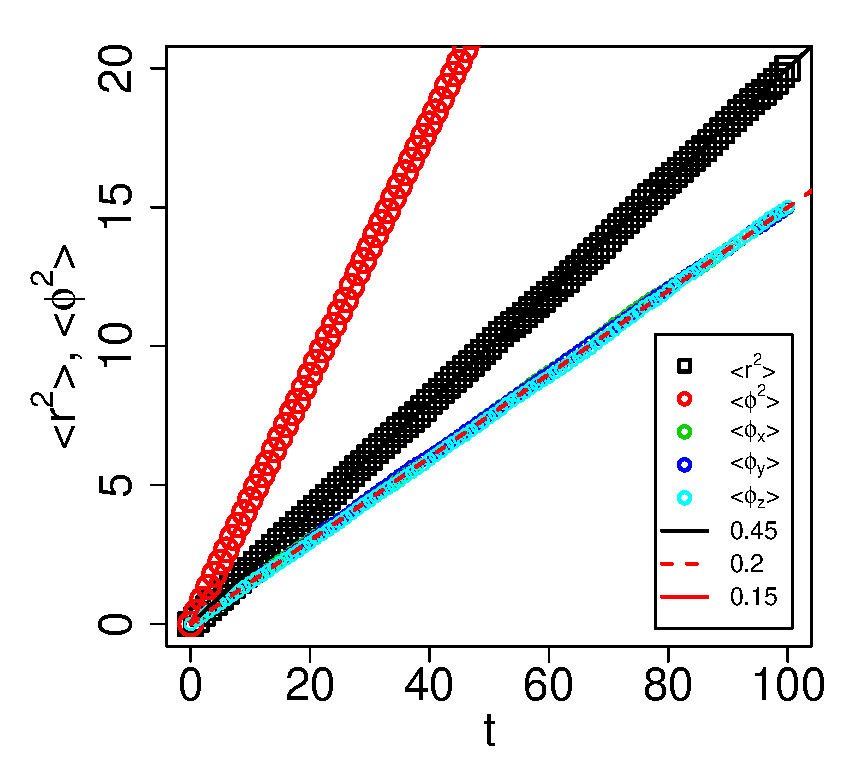
\includegraphics[height=0.3\textheight]{Images/DiffusionStats_drift}
	\captionsetup{justification=centering, width=0.9\textwidth}
	\caption{Particle MSD and RMSD (with components) as function of time. Points are obtained numerically, with averaging over $20000$ samples. Every sample started from $r_z = v_z = \omega_i = 0$ and particle co-aligned to $z$ axis. Solid lines are theoretical displacement (eqs. \eqref{eq:translation_diffusion_vs_displacement}, \eqref{eq:rotational_diffusion_vs_displacement}) for given $k_BT = 1$, $m = 1$, $R = 1$ and $\tau_t = 0.1$.}
	\label{fig:diffusion_stats_mean_square_displacement}
\end{figure}

Average kinetic energy per degree of freedom is $1/2 \, k_B T$, which for our case of full three-dimensional rotational and one-dimensional translational movement gives $E_k = 2 k_B T$

At equilibrium, velocity should satisfy Maxwell-Boltzmann distribution
\begin{equation}
\label{eq:maxwell_boltzmann_velocity}
	\begin{aligned}[c]
		p(v^2)
			= \sqrt{ \left(\frac{m}{2 \pi k_B T}\right)^3}
			4 \pi v^2 \exp \left[-\frac{mv_i^2}{2k_BT}\right]
	\end{aligned}
	\qquad
	\begin{aligned}[c]
		p(\omega^2)
			= \sqrt{ \left(\frac{I}{2 \pi k_B T}\right)^3}
			4 \pi \omega^2 \exp\left[-\frac{I\omega_i^2}{2 k_B T}\right]
	\end{aligned}
\end{equation}
where $v$ is translational and $\omega$ is rotational velocity, $m$ is particle mass, and $I$ is particle inertia, $k_B$ is Boltzmann constant and $T$ is thermodynamics temperature.

Velocity components should satisfy normal distribution 
\begin{equation}
\label{eq:maxwell_boltzmann_velocity_components}
	\begin{aligned}[c]
		p(v_i)
			= \sqrt{ \frac{m}{2 \pi k T}}
			\exp \left[-\frac{mv_i^2}{2kT}\right]
	\end{aligned}
	\qquad
	\begin{aligned}[c]
		p(\omega_i)
			= \sqrt{ \frac{I}{2 \pi k T}}
			\exp\left[-\frac{I\omega_i^2}{2kT}\right]
	\end{aligned}
\end{equation}

It can be shown that ratio between $\sigma^2_v = k_BT/m$ and $\sigma^2_\omega = k_BT/I$ is
\begin{equation}
\label{eq:velocity_deviation_relation}
	\frac{\sigma^2_v}{\sigma^2_\omega} = \frac{2}{3}R^2
\end{equation}
where $R$ is radius of a particle.

At the \figref{fig:velocity_distributions} the velocity probability distribution are shown, both theoretical and obtained from simulations, for one value of $k_BT = 1$ and $m = 1$. As expected, the $\sigma^2_v / \sigma^2_\omega$ are related as $2/3$ for our case of $R = 1$.

\begin{figure}[h]
\centering
	\begin{subfigure}[t]{0.45\textwidth}
		\centering
		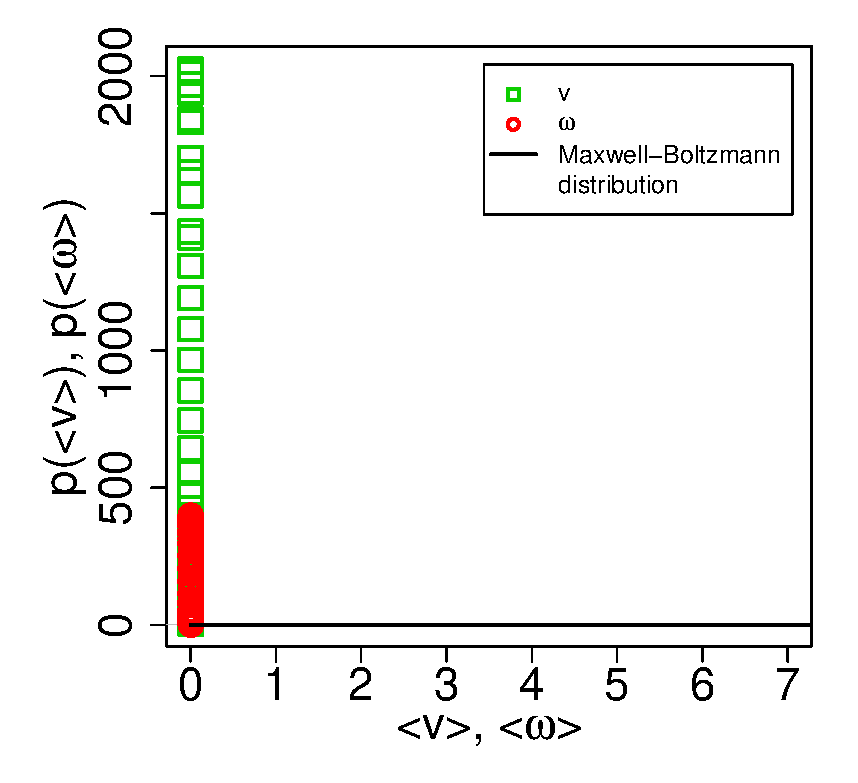
\includegraphics[width=\textwidth]{Images/DiffusionStats_mb}
		\captionsetup{justification=centering, width=0.9\textwidth}
		\caption{Probability distribution of velocity module. Theoretical distribution is given by equation~\eqref{eq:maxwell_boltzmann_velocity}}
	\end{subfigure}
	\begin{subfigure}[t]{0.45\textwidth}
		\centering
		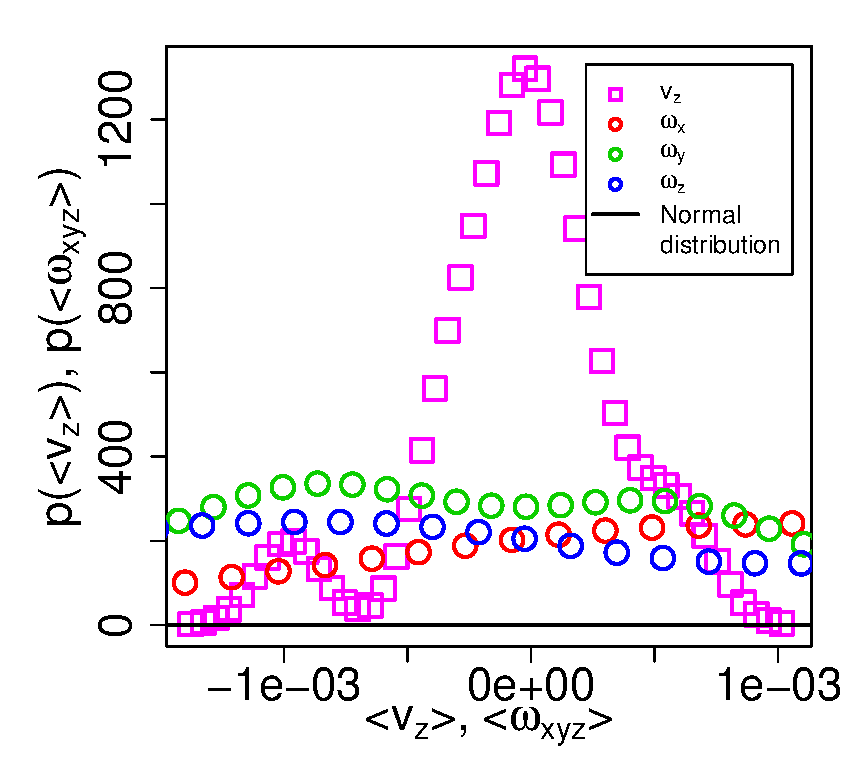
\includegraphics[width=\textwidth]{Images/DiffusionStats_norm}
		\captionsetup{justification=centering, width=0.9\textwidth}
		\caption{Probability distribution of velocity components. Theoretical distribution is given by equation~\eqref{eq:maxwell_boltzmann_velocity_components}}
	\end{subfigure}
	\captionsetup{justification=centering, width=0.9\textwidth}
	\caption{Translational and rotational velocity probability distribution. Points are obtained numerically, with averaging over $20000$ samples at time $t = 100$. Every sample started from $r_z = v_z = \omega_i = 0$ and particle co-aligned to $z$ axis. Solid lines are theoretical distributions for given $k_BT = 1$ and $m = 1$}
	\label{fig:velocity_distributions}
\end{figure}